

\documentclass[11pt]{amsbook}

\usepackage{../HBSuerDemir}	% ------------------------

\usepackage{wrapfig}

\begin{document}

% ++++++++++++++++++++++++++++++++++++++
\hPage{b2p1/229}
% ++++++++++++++++++++++++++++++++++++++

of the line $P_{0}P$ being $x-x_{0},y-y_{0},z-z_{0}$ or\\

\begin{center}
	
	$\frac{x-x_{0}}{t-t_{0}},\frac{y-y_{0}}{t-t_{0}},\frac{z-z_{0}}{t-t_{0}}$

\end{center}

their limits, as $t\rightarrow t_{0}$, are $x(t_{0}),y(t_{0}),z(t_{0})$ and are\par
components of a tangent vector at $P_{0}$. Hence

\begin{center}
    
    \begin{equation*}
        $r(t_{0})=(x(t_{0}),y(t_{0}),z(t_{0}))$
    \end{equation*}
    
\end{center}

is a \underline{tangent vector} to r at $P(t_{0})$, and

\begin{center}
    
    \begin{equation*}
        $r(t)=(x(t),y(t),z(t))$
    \end{equation*}
    
\end{center}

is a tangent vector at P(t). The differential

\begin{center}
    
    \begin{equation*}
        $dr = (x, y, z)dt$
    \end{equation*}
    
\end{center}

is also a tangent vector.\par
The vector of equation of the tangent line at $P_{0}$ is then

\begin{center}
    
    \begin{equation*}
        $P=P_{0}+ \lambda r(t_{0})$
    \end{equation*}
    
\end{center}



\begin{wrapfigure}{r}{2.5cm}
    
    
    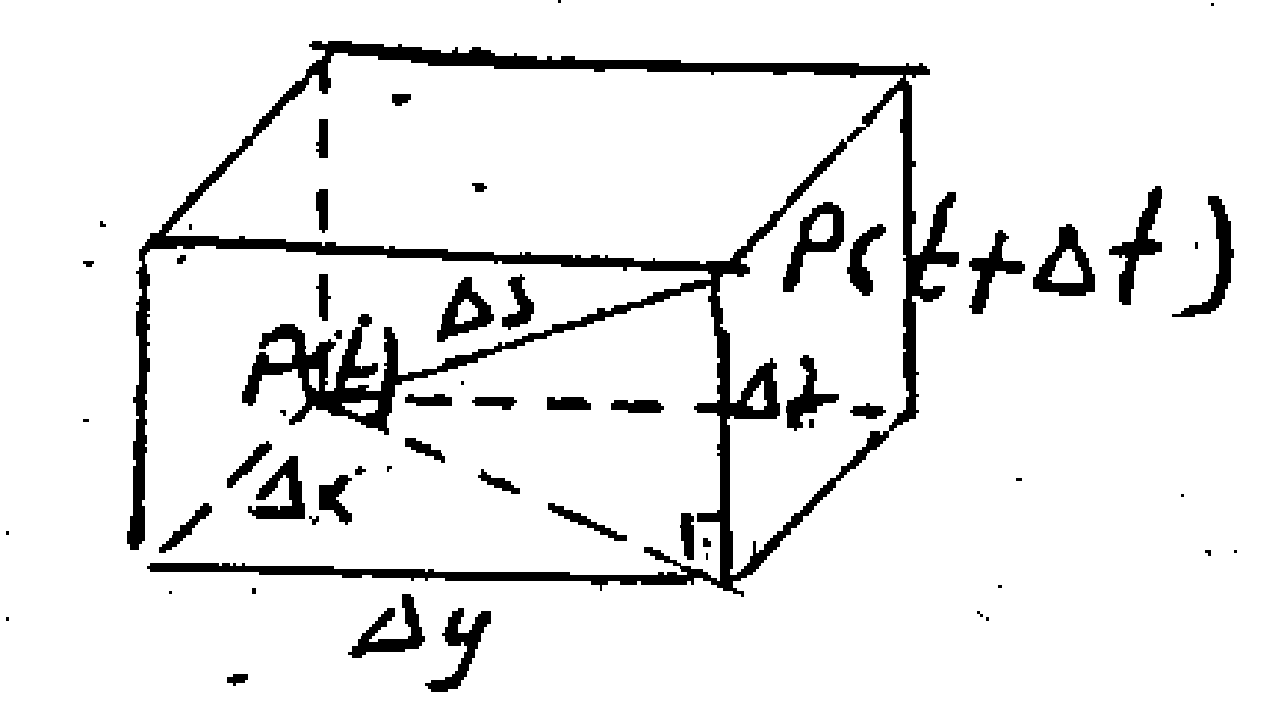
\includegraphics[width=4.5cm]{images/b2p1-229-fig01}

\end{wrapfigure} 

\begin{flushright}
    \footnote{Used wrapfig package for the figure.}
\end{flushright}

\underline{Arclength.}

Consider two nearby points\\
P(t) and $P(t+\Delta t)$\\
on r. The length $\Delta s$ of the chord\\
joining these points is an approximation\\
to the are from P(t) to $P(t+\Delta t)$. Now, from the figure
\vspace{-0.75cm}


\begin{equation*}
    
    $(\Delta s)^2=(x(t+\Delta t)-x(t))^2+(y(t+\Delta t)-y(t))^2+(z(t+\Delta t)-z(t))^2$\\
    $=\Delta x^2+\Delta y^2+\Delta z^2$\\
    $\Rightarrow (\frac{\Delta s}{\Delta t})^2 = (\frac{\Delta x}{\Delta t})^2+(\frac{\Delta y}{\Delta t})^2+(\frac{\Delta z}{\Delta t})^2$
    
\end{equation*}






% =======================================================
\end{document}  

%==== templates ====

%==== environments ====

%\begin{figure}[htb]
%	\centering
%	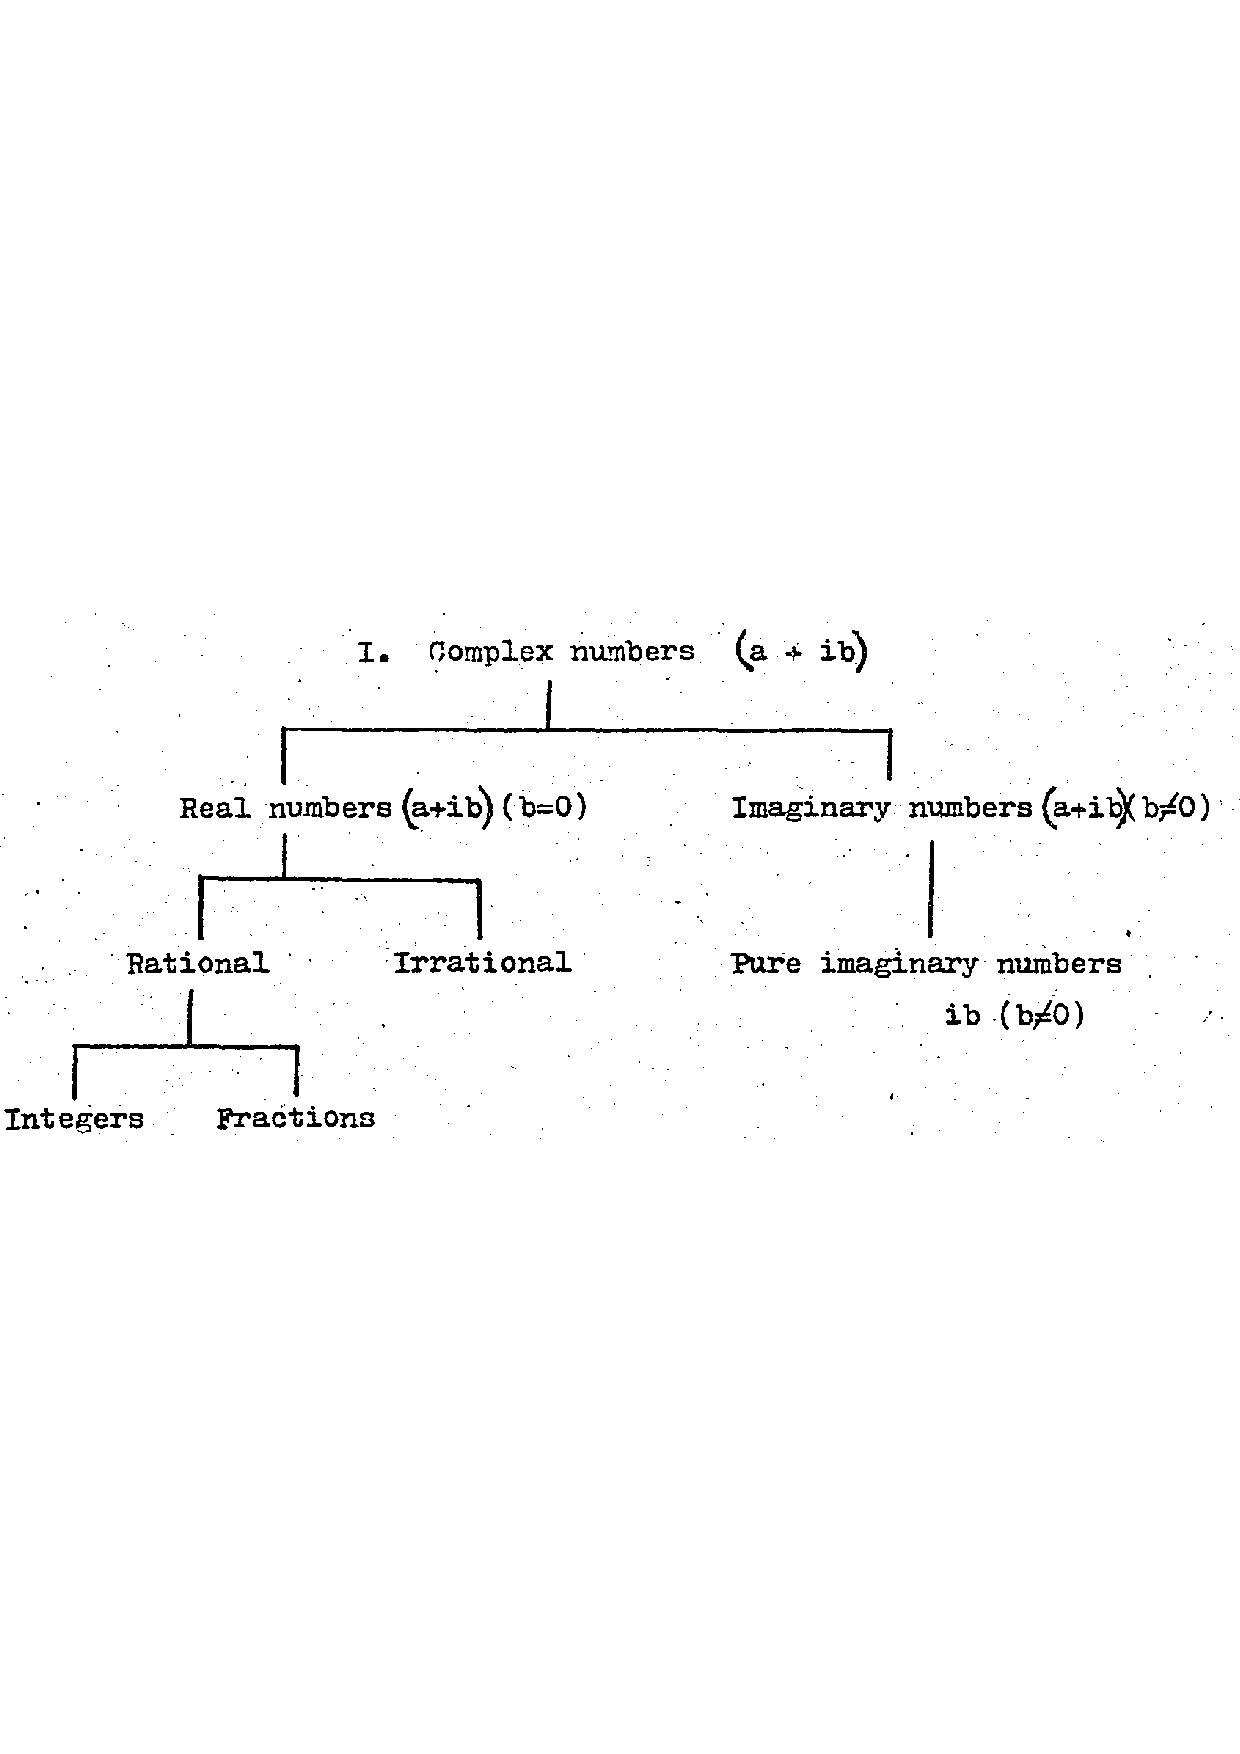
\includegraphics[width=0.9\textwidth]{images/SD-1-1p15A}
%	\caption{Classification of complex numbers}
%	\label{fig:classificationOfComplexNumbersA}
%\end{figure}

%\begin{center}
%\begin{tabular}{cc}
%\end{tabular}
%\end{center}

%\begin{exmp}
%\begin{hSolution}
%\end{hSolution}
%\end{exmp}

%\begin{hEnumerateAlpha}
%\end{hEnumerateAlpha}

%\begin{hEnumerateRoman}
%\end{hEnumerateRoman}

%$
%\begin{bmatrix}
%\end{bmatrix}
%$

%\frac{aaaa}{bbb}
%\frac{a_{n}}{b_{n}}
%\left( aaaa \right)
%\Longrightarrow

%\begin{multicols}{2}
%	bb
%\columnbreak
%	aa
%\end{multicols}
